\documentclass[sigconf,anonymous,10pt]{acmart}
\usepackage{graphicx}
\usepackage{booktabs}
\usepackage{amsmath,amssymb}
\graphicspath{{figures/}}

% Marker for results that land only after the 7-day run completes (2026-07-18).
% Remove this macro and its uses once the merged dataset is in and the numbers are filled.
\newcommand{\pending}{\textbf{[pending: 7-day run completes 2026-07-18]}}

%% Conference info — update when you have the official details from AINTEC
\acmConference[AINTEC '26]{Proceedings of the 21st Asian Internet Engineering Conference}{December 1--3, 2026}{Taipei, Taiwan}
\acmYear{2026}
\copyrightyear{2026}
\acmArticleSeq{8}
\begin{document}

\title{The Local Path Not Taken: Traffic Tromboning and Routing Inefficiency in Pakistan}

%% Authors are anonymised for double-blind review.
%% Remove the anonymous block and add real author info for camera-ready.
\author{Anonymous Author(s)}
\affiliation{%
  \institution{Anonymous Institution}
}
\email{anonymous@example.com}

\renewcommand{\shortauthors}{Anonymous et al.}

\begin{abstract}
Pakistan operates an Internet exchange, PKIX, in three cities with dozens of connected member
networks, yet its route server appears in none of the BGP paths we observe to Pakistani
destinations: the exchange is built but, for most traffic, not used. We measure the consequence
from inside the country. From every RIPE Atlas probe connected in Pakistan we run TCP traceroutes
and pings to a fixed, reproducibly sampled set of 100 Pakistani websites---stratified across
critical-infrastructure sectors and across local, CDN, and offshore hosting---once an hour and once
every half hour for a week, and we classify each path as domestic or hairpinned using a detector
grounded in round-trip-time physics rather than unreliable geo-IP. The uniform, longitudinal design
lets us report, on equal terms and per ISP, how much domestic traffic trombones abroad and through
which transit operators, what latency this costs and whether the cost is structural or diurnal,
and---from routing verdicts that flip between local and hairpinned across the week---whether a
domestic path exists for the traffic that nonetheless leaves the country. \pending{} The recurring
finding of the broader study is that the local path exists but is not taken, and that PKIX is the
instrument that would take it.
\end{abstract}

%%


%%
\begin{CCSXML}
<ccs2012>
<concept>
<concept_id>10003033.10003079.10011704</concept_id>
<concept_desc>Networks~Network measurement</concept_desc>
<concept_significance>500</concept_significance>
</concept>
<concept>
<concept_id>10003033.10003083.10003090.10003091</concept_id>
<concept_desc>Networks~Topology analysis and generation</concept_desc>
<concept_significance>300</concept_significance>
</concept>
<concept>
<concept_id>10003033.10003039.10003045.10003046</concept_id>
<concept_desc>Networks~Routing protocols</concept_desc>
<concept_significance>100</concept_significance>
</concept>
</ccs2012>
\end{CCSXML}

\ccsdesc[500]{Networks~Network measurement}
\ccsdesc[300]{Networks~Topology analysis and generation}
\ccsdesc[100]{Networks~Routing protocols}

\keywords{Internet exchange points, traffic tromboning, Pakistan, hairpinning, developing regions, PKIX, RIPE Atlas, latency, routing measurement}
\acmArticleSeq{8}
\maketitle

\section{Introduction}
Pakistan has 116 million internet users~\cite{datareportal2025pk}, yet a student submitting a university application, a citizen checking their tax records, or a small business owner processing a payment may find their request travelling thousands of kilometres to a server in Singapore or Frankfurt before returning to a destination that was never more than a few milliseconds away. This is not a failure of infrastructure in the conventional sense. Pakistan operates an internet exchange, PKIX, at three cities with dozens of member networks. The physical remedy exists. Yet for most Pakistani internet traffic, it is not being used.

The problem has a specific structure. Only two operators hold international gateway licences in Pakistan: PTCL and Transworld~\cite{pacra2023twa}. Every other ISP purchases upstream connectivity from one of them. When two Pakistani ISPs want to exchange traffic, they do so by peering, which means establishing a direct connection to hand off packets to each other rather than sending them through a third party. An internet exchange point provides a shared physical location where many networks can peer at once, avoiding the need for each pair to arrange a separate connection. Without peering at such an exchange, two ISPs in the same city will still route traffic through one of the two international operators, and those operators frequently send it abroad before it comes back. This is called traffic tromboning, and its consequences go beyond wasted milliseconds. When submarine cables fail, as they did during the SMW5 fault in July 2026 and six times in a single year in 2022~\cite{opalinski2024quest}, internationally-routed traffic degrades while locally-exchanged traffic is untouched. The country's dependence on foreign transit creates a resilience gap that a functioning exchange would close.

PKIX's own published figures show inter-ISP latency dropping from 100--144\,ms internationally to 1--31\,ms through the exchange~\cite{pta2026}. And yet the PKIX route server (AS140307) does not appear in a single BGP path we observe to Pakistani networks. The exchange is built, connected, and capable. It is simply not being used for most of the traffic that could benefit from it.

This paper measures the consequences of that underuse using active measurements from RIPE Atlas probes distributed across Pakistani ISPs. We run traceroutes and pings over a week-long window to 100 Pakistani websites spanning government, education, banking, news, and other sectors, and we classify each path using an RTT-physics detector that does not rely on geo-IP. Our three research questions are:

\begin{description}
  \item[RQ1] To what extent does Pakistani internet traffic trombone through foreign networks, and which ISPs and transit paths are responsible?
  \item[RQ2] What is the quantifiable RTT cost of tromboning, and is this penalty stable over time or does it vary with time of day or day of week?
  \item[RQ3] For destinations that trombone, does a local path demonstrably exist, evidenced by routing verdicts that flip between local and hairpinned across the measurement window?
\end{description}

Our findings show that the penalty is real, structural, and unevenly distributed across ISPs. More importantly, in most cases a local path already exists but is not chosen. The central argument of this paper is simple: Pakistan does not need to build new infrastructure to improve its internet routing. It needs to use what it already has.


\section{Background}
Di Bartolomeo et al.~\cite{dibartolomeo2015} compare IXP vs upstream paths for Italian ISPs
using RIPE Atlas and controlled BGP announcements, finding IXP paths give better, more stable
latency and preserve traffic locality; our study mirrors their vantage (national probes $\to$
national targets) and their locality-as-sovereignty framing, but replaces hand-picked targets
with a \emph{complete prefix census} and a detector that does not trust geo-IP. Gupta et
al.~\cite{gupta2014} show African ISPs that do not peer locally send domestic traffic
\emph{detouring through Europe}---precisely the tromboning we measure in Pakistan.
Prefix-based target selection follows the selective-scanning approach~\cite{klick2016}: all IPs
in an announced prefix share one BGP route, so a few IPs per block is routing-complete.
Large-IXP studies ~\cite{ager2012,chatzis2013} motivate why peering matters. We built on RIPEs Atlas~\cite{ripeatlas}, RIPEstat ~\cite{ripestat} and Team Cymru with an RDAP fallback for ASN
and registry resolution.

\section{Methodology}
\subsection{Site Selection}
\label{sec:sites}

We assembled a candidate pool of 1,814 Pakistani websites from three sources. First, we filtered the Tranco top-1 million domain ranking list~\cite{tranco} for domains ending in \texttt{.pk}, yielding 1,522 candidates. Tranco aggregates traffic data from Alexa, Majestic, Umbrella, and Quantcast and is designed for reproducible network measurement research. Second, we cross-referenced the Pakistan Telecommunication Authority's published list of licensed ISP operators to identify ISP corporate websites, retaining 86 valid domains after DNS resolution and manual verification. Third, we added healthcare sector sites and six PK-hosted sites identified during ASN lookup that were absent from the Tranco slice.

Each site was classified into one of three hosting categories. A site is \textit{Pakistani} if its IP resolves to a Pakistani ASN (country code PK) via Team Cymru bulk WHOIS lookup. It is \textit{CDN-hosted} if it resolves to a major content delivery network such as Cloudflare, Akamai, or Alibaba regardless of geographic location. It is \textit{Abroad} if it resolves to a foreign ASN that is not a CDN. Classification was performed programmatically using \texttt{socket.gethostbyname()} for DNS resolution followed by Team Cymru DNS-based ASN lookup.

Every site was then assigned to one of the nine critical infrastructure sectors defined by the US Cybersecurity and Infrastructure Security Agency (CISA)~\cite{cisa}, following the approach used in prior IXP peering measurement research~\cite{dibartolomeo2015}. Table~\ref{tab:cisa-sectors} shows representative sites per sector.

\begin{table}[t]
\caption{CISA sector categorization with example sites.}
\label{tab:cisa-sectors}
\begin{tabular}{ll}
\toprule
\textbf{CISA Sector} & \textbf{Example sites} \\
\midrule
Government Services \& Facilities & fbr.gov.pk, ecp.gov.pk \\
Education                         & nu.edu.pk, aiou.edu.pk \\
Communications                    & ptcl.com.pk, nayatel.com \\
Commercial Facilities             & dunya.com.pk, daraz.pk \\
Energy                            & lesco.gov.pk, wapda.gov.pk \\
Financial Services                & hbl.com, mcb.com.pk \\
Healthcare \& Public Health       & pmdc.pk, mohw.gov.pk \\
Transportation Systems            & pakrail.gov.pk, piac.com.pk \\
\bottomrule
\end{tabular}
\end{table}

A final set of 100 sites was selected using proportional random sampling with seed 42 for reproducibility. Each sector received a minimum of 2 slots, with the remaining 82 slots distributed proportionally to each sector's PK and CDN pool size. We weight by PK and CDN counts rather than total pool size because tromboning is relevant precisely for traffic that could be exchanged domestically; internationally-hosted sites are legitimately abroad and less informative for this question. Within each sector, slots were divided 40\% Pakistani, 40\% CDN-hosted, and 20\% internationally-hosted. Where a sector lacked sufficient sites of one hosting type, the shortfall was filled from whichever type had the largest remaining pool. Table~\ref{tab:sample-allocation} shows the final allocation.

\begin{table}[t]
\caption{Final 100-site sample allocation by CISA sector and hosting type.}
\label{tab:sample-allocation}
\begin{tabular}{lcccc}
\toprule
\textbf{Sector} & \textbf{Total} & \textbf{PK} & \textbf{CDN} & \textbf{Abroad} \\
\midrule
Commercial Facilities             & 60 & 24 & 24 & 12 \\
Government Services \& Facilities & 11 &  4 &  5 &  2 \\
Education                         & 10 &  4 &  4 &  2 \\
Communications                    &  7 &  3 &  3 &  1 \\
Financial Services                &  4 &  2 &  1 &  1 \\
Energy                            &  3 &  1 &  1 &  1 \\
Healthcare \& Public Health       &  3 &  1 &  1 &  1 \\
Transportation Systems            &  2 &  1 &  1 &  0 \\
\midrule
\textbf{Total}                    & \textbf{100} & \textbf{40} & \textbf{40} & \textbf{20} \\
\bottomrule
\end{tabular}
\end{table}

\begin{figure}[t]
  \centering
  \includegraphics[width=\columnwidth]{figures/fig_hosting_providers.pdf}
  \caption{Distribution of the 100 sampled sites by hosting provider.}
  \label{fig:hosting-providers}
\end{figure}

The full pipeline is available in the project repository. Running the three scripts in order on the same input files produces identical output.

\paragraph{Location verification.}
Because the hosting classification above rests on geo-IP, we verify it against physics once
measurements are available: no reply can arrive faster than light in vacuum would need for the
round trip to a site's claimed location, so any measured RTT below that bound proves the claimed
location wrong. Applied to the first days of the panel, this test invalidated the registered
locations of 34 of the 40 CDN-class sites (anycast addresses whose registration city is, e.g.,
Toronto, yet which answer Pakistani probes in under 3\,ms) and corrected six unicast sites: three
sites classed as Pakistani-hosted were in fact far from every probe (nearest ping over 200\,ms,
consistent with their US and Singapore geo-IP) and are reclassified as Abroad, and three sites
whose claimed city was physically impossible were relocated by latency multilateration, using each
probe's RTT as a distance bound. The corrected hosting split is therefore 37 Pakistani, 40 CDN,
and 23 Abroad, and all per-class results below use the corrected classes. We treat this not as a
flaw in the sample but as a finding in its own right---among the misclassified sites is a
provincial government service hosted in the United States---and as independent validation that
registration-based location data cannot be trusted at exactly the addresses this study cares
about.

\subsection{Vantage Points}
We measure from the RIPE Atlas probes connected within Pakistani networks at the time of the run,
enumerated live from the platform API (country code PK, connected status) rather than from a fixed
list, so that the vantage set reflects whichever probes are actually online; at the launch of the
week-long run reported here this comprised 17 probes, of which 16 returned data (one probe, on the
state operator NTC, was offline throughout). We additionally verified each probe's metadata against
the platform API at analysis time rather than trusting run-time labels: one probe's stored label
carried a wrong autonomous-system number and was corrected (it is a Z-Com vantage), and one probe
declares a placeholder coordinate and is excluded from all distance-based analysis while its
round-trip times, which remain valid, are retained elsewhere. The probes span both licensed
international operators and a range of their downstream ISPs---PTCL and Transworld together with
its retail arm, alongside Cybernet, Nayatel, Nova, Orbit, and Z-Com among others---and, crucially
for RQ2, several ISPs contribute more than one probe and in more than one city, which is what lets
us ask whether the customers of a single ISP receive the same service. Three probes require care:
two are ICMP-filtered, so their intermediate hops do not respond and only their ping RTT is
trustworthy, and one runs inside a container that exposes only two hops. We retain the round-trip
time these probes report, since it remains valid, but exclude them from any hop-count statistic,
and we flag them wherever they enter an analysis rather than dropping them silently.

\subsection{Measurement Design}
Against each of the 100 sites we run two complementary measurements. A TCP traceroute to port~80
records the forward path and per-hop round-trip time once per hour, and an ICMP ping records
end-to-end RTT and packet loss every thirty minutes; both fan out to all connected probes, and both
run continuously for a seven-day window. We use TCP to port~80 rather than ICMP for the path because
ICMP is heavily filtered in Pakistani networks---on an earlier target only 12 of 52 destinations
answered ICMP at all---whereas a web server on port~80 is far more likely to reply, and we use
Paris-style traceroute, which holds constant the header fields a load balancer hashes on, so that a
change in the observed path is a genuine reroute and not an artefact of multipath forwarding. From
the ping series we take round-trip time to be the \emph{minimum} of the packets in a round rather
than the mean, because network noise is one-directional---a packet can be delayed by queuing but
never delivered faster than the path physically allows---so the minimum is the cleanest estimate of
the true latency. We report jitter as the standard deviation of RTT across rounds and packet loss as
the fraction of probe packets that go unanswered; together with hop count from the traceroute, these
give the four indicators used throughout, matching the metric set of prior IXP measurement
work~\cite{dibartolomeo2015}.

The measurements are registered with RIPE Atlas as server-side \emph{periodic} instructions with a
fixed start and stop, so that collection continues on the platform's own infrastructure independent
of our host and a local collector can be restarted without loss of data. RIPE Atlas caps the number
of simultaneously running measurements at one hundred per account; because one hundred sites each
require both a traceroute and a ping, the run needs two hundred concurrent measurements, which we
accommodate by splitting it across two credit-sharing accounts \emph{by measurement type}---one
account carrying all one hundred traceroutes and the other all one hundred pings, against the
identical site list and the same live-discovered probes. As the split is by type rather than by
site, the merged dataset is identical to what a single unconstrained account would have collected.
The credit and result-volume ceilings are an order of magnitude above what the run consumes, so
concurrency, not cost, is the only binding limit.

\subsection{The Latency Ratio}
\label{sec:ratio}
To compare connections fairly across distances, we normalise each measured round-trip time by the
fastest round trip physics allows for that connection, giving a dimensionless \emph{latency
ratio}: a value of $1$ means the path performs at its physical limit, and a value of $k$ means the
connection takes $k$ times longer than the best possible. Because the ratio is unitless it can be
pooled across near and far sites and plotted as a distribution, and we retain the hosting class of
every site so the distributions can be sliced by type. The theoretical minimum differs by class.

For \textbf{unicast sites} (the Pakistani and Abroad classes, one physical server each), the
minimum is set by geography. With the probe and server coordinates, the great-circle distance $d$
follows from the Haversine formula, and light in optical fibre covers it at
$v_f = c/1.468 \approx 204{,}200$\,km/s, so
\begin{equation}
  \mathit{RTT}_{\min} \;=\; \frac{2d}{v_f} \;\approx\; \frac{d~[\mathrm{km}]}{102}~\mathrm{ms},
  \qquad
  \text{ratio} \;=\; \frac{\mathit{RTT}_{\mathrm{measured}}}{\mathit{RTT}_{\min}},
\end{equation}
where $\mathit{RTT}_{\mathrm{measured}}$ is the minimum ping over the window (noise only ever adds
delay, so the minimum best approximates the true path latency). Probe coordinates come from the
platform API; server coordinates from the verified geo-IP of the measured address
(\S\ref{sec:sites}). Pairs closer than 30\,km are excluded from the ratio---the denominator
approaches zero and the quotient degenerates---and are reported directly in milliseconds instead
(their median in our data is 6\,ms, i.e.\ same-city delivery is healthy).

For \textbf{CDN sites} no single server location exists: the same anycast address is served from
different points of presence for different ISPs, and its registered location is provably wrong
(\S\ref{sec:sites}). We therefore define the theoretical minimum \emph{empirically}: the best RTT
that any Pakistani probe achieves to that site. This floor is attainable by construction---any ISP
could peer with the best-performing network, at the exchange this paper is about, and match its
path---so the ratio
\begin{equation}
  \text{ratio}_{\mathrm{CDN}} \;=\;
  \frac{\mathit{RTT}_{\mathrm{measured}}(\mathrm{probe}, s)}
       {\min_{\mathrm{all\ probes}} \mathit{RTT}_{\mathrm{measured}}(\cdot\,, s)}
\end{equation}
measures exactly what an ISP loses by not peering. It contains no distance and no geo-IP; the
best-connected ISP scores $1$ and defines the frontier.

\subsection{Tromboning Classification}
\label{sec:detector}
To decide whether a given trace left the country we rely on the round-trip time recorded at each hop
rather than on the registration country of the hop's IP address, because geo-IP is wrong at exactly
the hops that matter. Two of the addresses that appear most often in Pakistani paths---a Shaw block
registered to Canada and a Cogent block registered to the United States---in fact sit physically in
Pakistan and answer in about two milliseconds, so a country-of-registration test would misread them
as foreign; conversely, a genuinely foreign exit, such as Transworld's egress at an exchange in
Singapore, is frequently unannounced in BGP and carries no reliable country at all. We therefore
classify by RTT physics. A trace is judged to have left Pakistan if any responding hop that is not
in the country answers at 40\,ms or more, or if the RTT jumps by at least 60\,ms between consecutive
hops, or if any hop answers at 70\,ms or more; a trace whose maximum RTT stays below 45\,ms is
classified as local. The 40\,ms floor is the physical round-trip to the nearest international
exchange, and the jump rule catches foreign hops that do not themselves resolve. We discard
individual hop RTTs above 500\,ms as queuing or ICMP-error-generation artefacts, common on the
filtered probes, and we exclude the Shaw and Cogent addresses from country attribution.

We calibrated these thresholds against hop-by-hop RTT profiles inspected by hand. On an early ISP a
naive geo-IP classifier labelled all 53 measured paths as foreign, whereas the RTT-physics rules
identified 16 of 52 as hairpinned, in agreement with manual inspection; the remaining paths stayed
local through an in-country Cogent point of presence. Establishing this agreement before quoting any
tromboning rate follows the validation-before-evaluation norm of measurement work, and we carry the
same, unchanged detector through every result below so that the panel's verdicts are directly
comparable across ISPs and over time.

\section{Results}
\label{sec:results}
The week-long run is in collection at the time of writing; its window closes on 18~July~2026,
after which the traceroute and ping halves are merged on probe, site, and round, and the three
analyses the panel is designed for---one per research question---are computed on the full week
(\S\ref{sec:rq1}--\S\ref{sec:rq3} below). Ahead of that, we report two supporting analyses from a
snapshot taken three days into the window. They serve two purposes: they exercise the full
pipeline of \S3 end to end, and---because every number below is a minimum over rounds, which
additional days can only tighten---they establish stable baselines that the full-week results will
refine rather than overturn. Both are labelled preliminary.

\subsection{Preliminary: Latency Ratio by Site Type}
\label{sec:prelim-ratio}
Figure~\ref{fig:ratio-cdf} shows the distribution of the latency ratio (\S\ref{sec:ratio}) for the
507 probe--site connections to unicast sites with a ping response and the 617 connections to CDN
sites, as cumulative distribution functions. Three observations stand out. First, connections to
\emph{foreign} sites are the control group the metric needs: their ratios are tight (median
2.5$\times$, none beyond ${\sim}7\times$), showing what ordinary routing achieves when it works.
Second, connections to \emph{Pakistani} sites match that typical performance (median 2.9$\times$)
but roughly a third of them tail out to 10--30$\times$---inefficiency that, given the control
group, cannot be blamed on ordinary Internet overhead and sits exactly where domestic detours
live; the full-week traceroutes attribute these paths in \S\ref{sec:rq1}. Third, the \emph{CDN}
curve is bimodal: about a third of ISP--site pairs sit at ${\approx}1\times$ (those ISPs ride the
locally peered path and define the floor), while roughly a quarter exceed 40$\times$. Access to
anycast content is effectively binary---an ISP either peers locally or hauls the traffic to a
distant point of presence---which previews the cross-section of the next subsection. One caveat
qualifies the Pakistani curve: 22 of the 40 Pakistani-class sites drop ICMP and are absent here;
they will be filled in from the TCP traceroute half of the panel, whose final hop the web servers
must answer.

\begin{figure}[t]
  \centering
  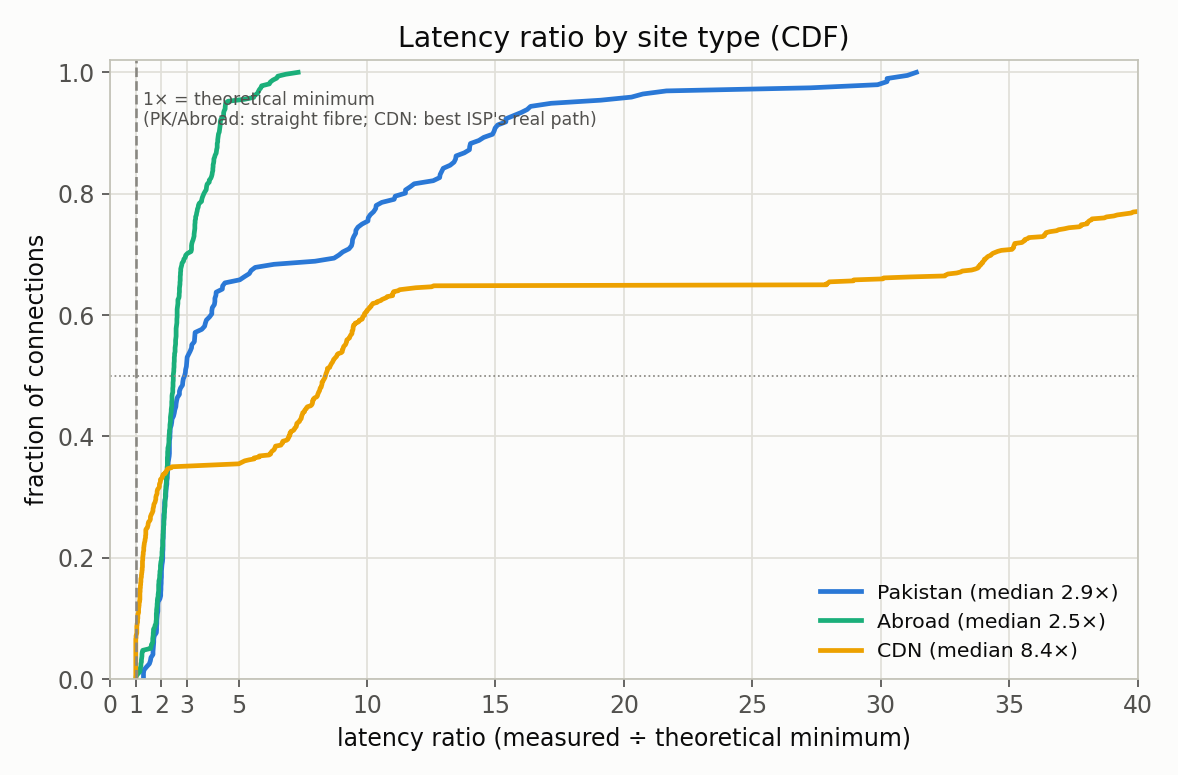
\includegraphics[width=\columnwidth]{ratio_cdf_all3.png}
  \caption{Latency ratio by site type (snapshot, first three days). For Pakistani and Abroad sites
  the theoretical minimum is straight fibre over the verified great-circle distance; for CDN sites
  it is the best RTT any Pakistani probe achieves (\S\ref{sec:ratio}). Foreign sites are uniform;
  Pakistani sites carry a long tail; CDN access is bimodal.}
  \label{fig:ratio-cdf}
\end{figure}

\subsection{Preliminary: The CDN Cross-Section---the Local Path Exists}
\label{sec:prelim-cdn}
RQ3 asks whether a local path exists for traffic that nonetheless leaves the country, and answers
it longitudinally, through verdicts that flip over the week. The CDN measurements already answer
the same question \emph{cross-sectionally}. Figure~\ref{fig:cdn-heatmap} shows, for each ISP and
each CDN-hosted site, how close the point of presence that serves that ISP is: local
($<$15\,ms), regional (15--50\,ms), or far ($>$50\,ms), thresholds we calibrated in earlier
cache-presence work. The rows order themselves into a peering ranking: the best-peered network
reaches 85\% of CDN content locally at a median of 3\,ms, two others reach 41\% and 20\%, and the
remaining six ISPs---including the largest operator---reach essentially none of it locally,
with medians up to 136\,ms. Expressed with the CDN ratio of \S\ref{sec:ratio}, the median cost of
non-peering ranges from $2\times$ (second-best network) to $52\times$ (the largest operator): the
same national content, in some cases military and provincial-government sites, is tens of times
slower depending only on which ISP a citizen uses. The columns separate causes: sites red across
\emph{every} row are far because of their own offshore fronting (no peering can fix them), whereas
columns green for well-peered ISPs and red for the rest quantify precisely the local path that
exists and is not taken. This is the paper's thesis in cross-section; the longitudinal version
follows on the full week in \S\ref{sec:rq3}.

\begin{figure}[t]
  \centering
  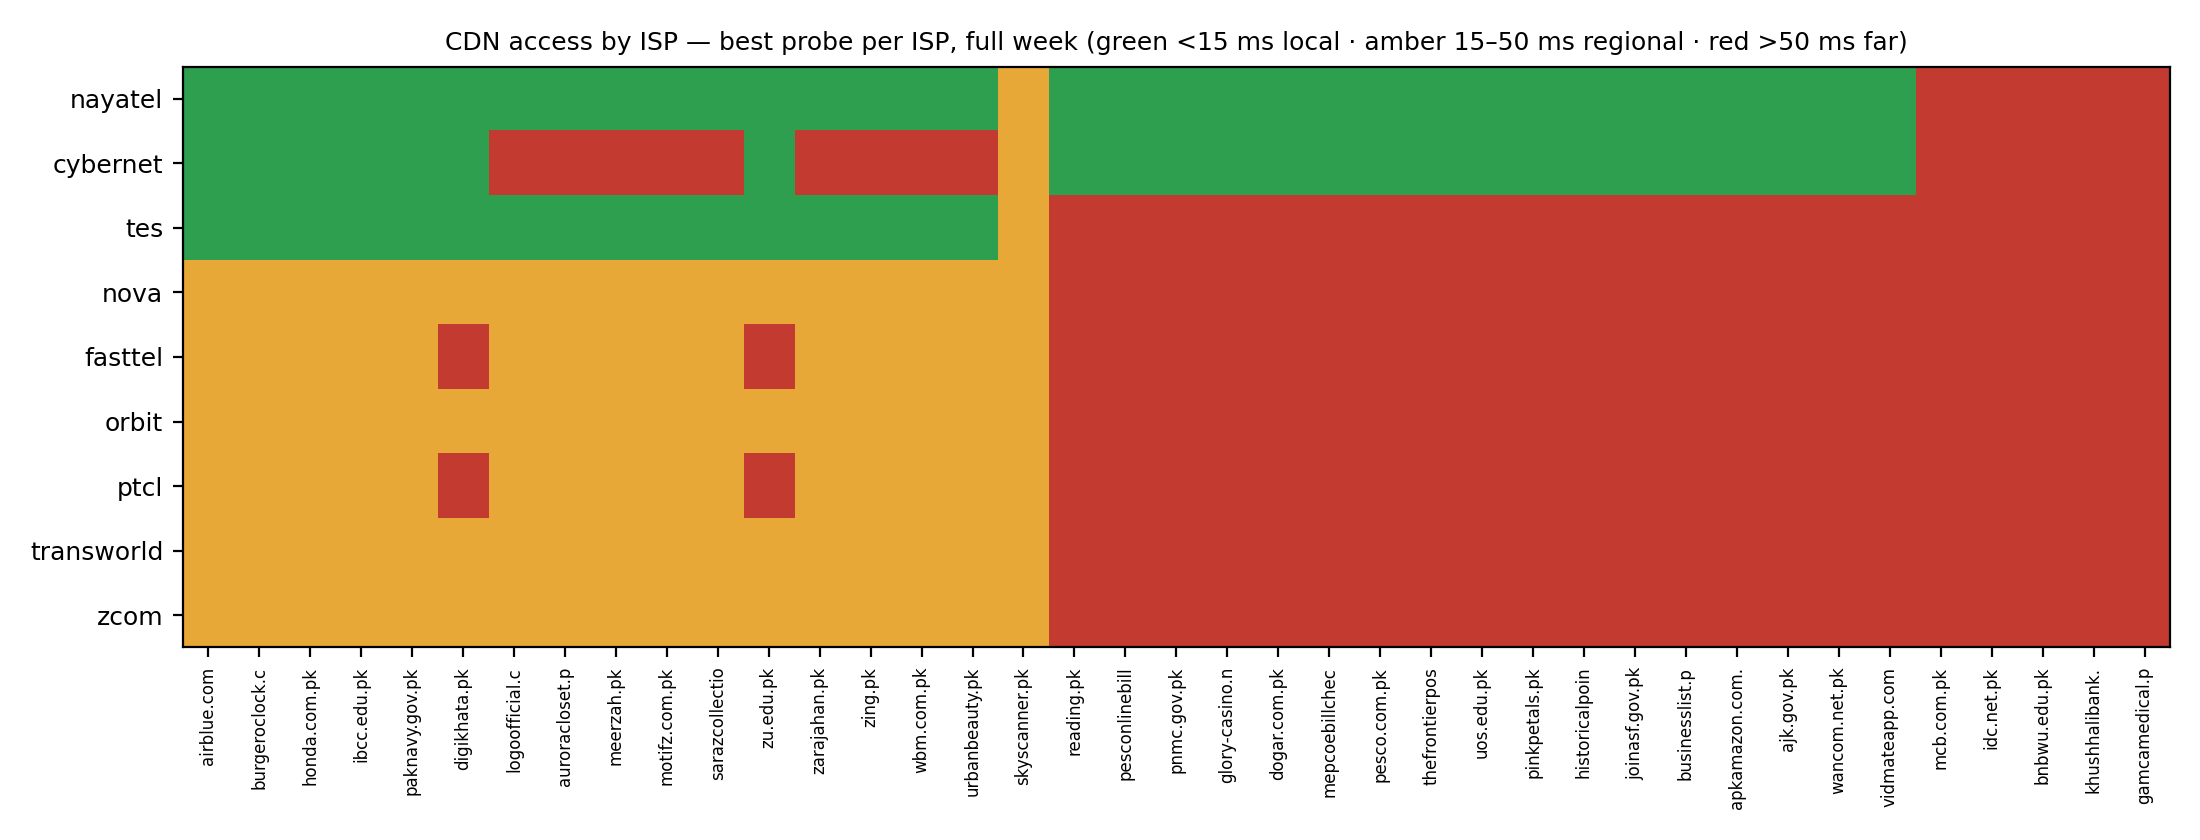
\includegraphics[width=\columnwidth]{cdn_heatmap.png}
  \caption{CDN access grid (snapshot, best probe per ISP). Green: served from a local PoP
  ($<$15\,ms); amber: regional (15--50\,ms); red: far ($>$50\,ms). Rows form a peering ranking;
  solid-red columns are sites fronted offshore for every ISP.}
  \label{fig:cdn-heatmap}
\end{figure}

\subsection{Extent and Attribution of Tromboning (RQ1)}
\label{sec:rq1}
For each ISP we will report the fraction of its traces to Pakistani-hosted sites that leave the
country, broken down both by the transit operator that performs the hand-off abroad and by the exit
country at which the path leaves. Because the panel measures every hour for a week rather than once,
it separates an ISP that hairpins persistently from one that does so only intermittently, and
because it measures from every connected probe, it tests whether the outcome is governed more by the
vantage---the ISP, and even the specific point of presence one measures from---than by the
destination. We present the per-ISP rates as a ranked bar chart and the hand-off attribution as a
stacked breakdown by transit operator and exit country, the direct analogue of the
foreign-AS-traversal figure in prior IXP work~\cite{dibartolomeo2015}.
% \begin{figure}[t]\centering\includegraphics[width=\columnwidth]{fig_panel_trombone_by_isp.png}
%   \caption{Tromboning rate per source ISP, with transit/exit attribution.}\label{fig:panel_source}\end{figure}
\emph{Reserved:} per-ISP trombone rate; transit (PTCL/Transworld) and exit-country attribution. \pending

\subsection{The Latency Cost and Its Stability (RQ2)}
\label{sec:rq2}
We will present the distribution of round-trip time for local versus hairpinned traces as cumulative
distribution functions, both pooled and per ISP, so that the cost of tromboning is expressed as a
full distribution rather than a single mean; a clean separation between the two curves is the
quantitative statement of the penalty. Because the measurement spans a full week at fine cadence, we
then decompose that penalty by time of day and day of week to test whether it is a fixed structural
cost or one that rises with evening congestion. A flat profile would show the penalty to be a
consequence of where content is hosted and how it is routed, not of load, and therefore that the
remedy is local hosting and peering rather than additional capacity; a pronounced cycle would
instead localise when the cost is worst. The preliminary ratio distributions of
\S\ref{sec:prelim-ratio} are the partial-window baseline this analysis refines: the full week adds
the diurnal decomposition and the per-ISP split, and a path-only variant that subtracts each
probe's measured last-mile floor (on the snapshot, the Pakistani median falls from 2.9$\times$ to
1.9$\times$, below the foreign 2.4$\times$, indicating the typical domestic route is efficient and
the cost lives in the access overhead and the tail).
% \begin{figure}[t]\centering\includegraphics[width=\columnwidth]{fig_panel_rtt_cdf.png}
%   \caption{CDF of min-of-$N$ RTT, local vs hairpinned traces.}\label{fig:panel_cdf}\end{figure}
\emph{Reserved:} RTT CDF (local vs hairpinned, pooled and per ISP); diurnal/weekly penalty curve. \pending

\subsection{Existence of a Local Path (RQ3)}
\label{sec:rq3}
Finally, for every Pakistani-hosted site that ever trombones we will report the fraction of the
week's rounds in which its verdict is local rather than hairpinned. A site whose verdict flips
between the two over the window is direct evidence that a domestic path exists and is sometimes
taken, so that the international detour on the remaining rounds is a routing \emph{choice} rather
than a necessity; a site that trombones on every round, by contrast, indicates no usable local path
from that vantage. Classifying each site as persistently local, persistently hairpinned, or flapping
turns the question of whether the local path exists into a measured quantity, and it lets us state
the tromboning rate as a range across the week rather than as a single fragile snapshot.
\emph{Reserved:} per-site verdict-flip fraction; persistently-local / persistently-hairpinned / flapping counts. \pending

\section{Discussion}
The measurement is built to support one argument, and its shape is already visible in the design. If
the penalty for reaching domestic content over an international detour is large and, as we expect,
stable across the day, then it is not a capacity problem that more bandwidth would solve but a
routing and hosting problem that local exchange would; and if the same destinations are reached
locally on some rounds and abroad on others, then the domestic path plainly exists and is simply not
being chosen. PKIX is the instrument that would choose it. The exchange is already present in three
cities with dozens of connected members, and its own figures put inter-ISP latency through the
exchange one to two orders of magnitude below the international alternative~\cite{pta2026}; the gap
our measurements probe is therefore not between the status quo and a network that must be built, but
between the status quo and one that must be \emph{used}. In the language of a three-set framing---
networks absent from the exchange, networks present but not exchanging routes, and networks actively
peering---the tromboning we measure is a picture of the first two behaviours at national scale, and
moving networks into the third is a matter of configuration and commercial willingness rather than
construction. The preliminary cross-section of \S\ref{sec:prelim-cdn} already shows what moving
between sets is worth: the same anycast content is a median $52\times$ slower on the largest
operator than on the best-peered network in the same country, a gap closable by peering rather
than by capacity.

The same structure explains the resilience concern that motivates the study. Because
internationally-routed traffic depends on a small number of submarine cables reached through the two
licensed gateways, a cable fault degrades precisely the traffic that need not have gone abroad,
while traffic hosted and exchanged domestically is untouched; the July~2026 SMW5 fault, during which
international paths grew erratic while local ones held, is a concrete instance. A functioning
exchange narrows this exposure directly, by keeping domestic traffic domestic.

Two limitations bound these claims. First, RIPE Atlas measures latency and paths but not traffic
volume, so we quantify the per-path cost of tromboning and not its aggregate economic cost---the
foreign transit purchased and the associated outflow of foreign exchange---which would require
volume data we do not have; we therefore leave a traffic-weighted estimate to future work. Second, a
low traceroute RTT to a CDN edge shows only that the network \emph{edge} is local, not that the
content is served locally, since a request may still be fulfilled from a distant point of presence;
we treat the CDN class accordingly and do not read a local edge as proof of local service.

\section{Conclusion}
Measured from inside the country, Pakistan's internet routing sends a substantial share of domestic
traffic abroad even though a domestic exchange exists to keep it home. This paper has presented the
design of a week-long, uniform measurement from every connected Pakistani vantage to a fixed,
reproducibly sampled set of one hundred sites, together with a geo-IP-independent classifier for
detecting when a path leaves the country, built to answer three questions: how much traffic
trombones and through whom, what that costs and whether the cost is structural, and whether a local
path exists for the traffic that takes the detour. The measurement is in collection; its results,
reported per ISP and over the full week, will quantify the extent, the cost, and the avoidability of
the detour. Preliminary analyses from the first days already validate the pipeline and preview the
answer: foreign sites are reached uniformly near the physical optimum, domestic sites carry a long
inefficiency tail, and the same CDN content varies by a factor of fifty between well-peered and
poorly-peered ISPs. The throughline is that the remedy is already in place: Pakistan does not need
to build new infrastructure to keep its traffic local; it needs to use the exchange it has. Beyond
this run, the same framework extends to a longer horizon, to repeated measurement that ranges the
tromboning rate over time, and---by holding a continuous normal-day baseline---to capturing the
next cable fault as a clean before-during-after rather than, as before, against an already-degraded
state.

\bibliographystyle{ACM-Reference-Format}
\bibliography{references}


\end{document}
